\documentclass[a4paper]{article}
\usepackage[affil-it]{authblk}
%\usepackage[backend=bibtex,style=numeric]{biblatex}
\usepackage{graphicx} % Required for inserting images
\usepackage{caption}
\usepackage[UTF8]{ctex}
\usepackage{epstopdf}
\usepackage{amsfonts,amssymb}
\usepackage{tikz}
\usetikzlibrary{chains}
\usepackage{listings}
\usepackage{xcolor}
\usepackage{float}
\usepackage{hyperref}
\usepackage{bookmark}
\usepackage{color}
\usepackage{verbatim}
\usepackage{subfig}
\usepackage{listings}
\lstset{
basicstyle=\ttfamily,
breaklines=true
}
% \usepackage{matlab-prettifier} % MATLAB 美化包
% \lstset{
%         style=Matlab-editor,
%         numbers      = left,
%         frame        = single,
% }
\usepackage{amsmath}
\usepackage{chngcntr}
\usepackage{pgfplotstable}
\pgfplotsset{compat=1.18}
\usepackage{makecell}
\usepackage{booktabs}      % 提供更好看的表格线
\usepackage{adjustbox}     % 用于调整表格大小
% \usepackage{csvsimple}
\counterwithout{equation}{section}
\counterwithout{figure}{section}

\usepackage{geometry}
\geometry{margin=1.5cm, vmargin={0pt,1cm}}
\setlength{\topmargin}{-1cm}
\setlength{\paperheight}{29.7cm}
\setlength{\textheight}{25.3cm}

\newcommand{\subsubsubsection}[1]{\paragraph{#1}\mbox{}\\}
\setcounter{secnumdepth}{4} % how many sectioning levels to assign numbers to
\setcounter{tocdepth}{4} % how many sectioning levels to show in ToC

\begin{document}
\begin{sloppypar}
% =================================================
\title{NA Project Design}

\author{陈澎 Chen Peng 3220103443
  \thanks{Email: \texttt{cpzju@zju.edu.cn}}}
\affil{Xinji 2201, Zhejiang University }

\date{\today}

\maketitle

% ============================================
\section{Program Design}
\subsection{Program Structure Description}
The design of the program is based on the object-oriented programming paradigm.
The program is divided into several classes, each of which is responsible for a
specific task. The classes are designed to be independent of each other, with
each class providing a specific interface for other classes to call.

The directory structure is as follows:
\begin{lstlisting}
project_code
|- doc % directory for documentation
|- figure % directory for figures
|- output % directory for output files like data
|- src % directory for source code
|- Makefile
\end{lstlisting}

The \verb|Makefile| is used to compile and run the source codes and generate the documents. 
Use \verb|c++11 -O3 -march=native| to speed up. Since Eigen3 compilation is relatively slow, please be patient and wait for 2-3 minutes.

The directory structure of doc is as follows:
\begin{lstlisting}
doc
|- design.tex % Tex file for program design
|- report.tex % Tex file for program execution report
\end{lstlisting}

The directory structure of figure is as follows:
\begin{lstlisting}
figure
|- intersect
|- problemA
|- problemC
|- problemE
|- problemF
|- requirement5
|- test
\end{lstlisting}
Each subdirectory contains figures for a specific problem or requirement.

The directory structure of output is as follows:
\begin{lstlisting}
output
|- intersect
|- problemA
|- problemC
|- problemD
|- problemE
|- problemF
|- requirement5
|- test
\end{lstlisting}
Each subdirectory contains output files for a specific problem or requirement.

The directory structure of src is as follows:
\begin{lstlisting}
output
|- intersect
    |- intersect_test.cpp
    |- plotIntersect.py
|- packages 
    |- eigen-3.4.0 % directory for Eigen library
    |- Function.hpp
    |- NodeType.h
    |- SplineType.h
    |- BoundaryCondition.h
    |- PPForm.hpp
    |- BSpline.hpp
    |- CurveFitting.hpp
    |- Intersection.hpp
|- problemA
    |- A.cpp
    |- plotA_leastSquare.py
    |- plotA.py
|- problemC
    |- C.cpp
    |- plotC.py
|- problemD
    |- D.cpp
|- problemE
    |- E_detailed_output.cpp
    |- E.cpp
    |- plotE_error.py
    |- plotE.py
|- problemF
    |- F.cpp
    |- plotF_divide.py
    |- plotF_trunc.py
|- requirement5
    |- plotRequire5.py
    |- requirement5.cpp
|- test
    |- plotTest.py
    |- test.cpp
\end{lstlisting}

Apart from the packages folder, each subdirectory contains source codes for a
specific problem or requirement.

\subsection{Explanation of Relationships Between Classes}
The packages consists of the following files:
\begin{itemize}
  \item \texttt{Function.hpp}
  \item \texttt{NodeType.h}
  \item \texttt{SplineType.h}
  \item \texttt{BoundaryCondition.h}
  \item \texttt{PPForm.hpp}
  \item \texttt{BSpline.hpp}
  \item \texttt{CurveFitting.hpp}
  \item \texttt{Intersection.hpp}
\end{itemize}

The \verb|Function.hpp| file is used to pass function objects and was
implemented in a previous course. We will not introduce the header file below.

The \verb|NodeType.h|, \verb|SplineType.h|, and \verb|BoundaryCondition.h|
files define three enumeration types:
\begin{itemize}
  \item \verb|NodeType|: Defines the types of node preprocessing, including Equidistant and ChordalLength.
  \item \verb|SplineType|: Defines the types of splines, including Piecewise Polynomial Form (PPForm) and B-Spline.
  \item \verb|BoundaryCondition|: Defines the types of boundary conditions for B-Splines, including PERIODIC, NATURAL, COMPLETE, NOT\_A\_KNOT, and SECOND.
\end{itemize}
These enumeration types provide configuration options for other files.

The \verb|PPForm.hpp| file defines a template class \verb|PPForm| for
representing Piecewise Polynomial Form. This class has two specializations for
fitting one-dimensional linear splines and cubic splines under five different
boundary conditions. It includes \verb|BoundaryCondition.h|.

The \verb|BSpline.hpp| file defines a template class \verb|BSpline| for
representing B-Splines. This class has three specializations for fitting
one-dimensional linear B-Splines, second-order B-Splines, and cubic B-Splines
under five different boundary conditions. It also implements B-Spline fitting
given known coefficients, knot sequences, and order conditions. It includes
\verb|BoundaryCondition.h|.

The \verb|CurveFitting.hpp| file defines a class \verb|CurveFitting| for curve
fitting. This class implements fitting for planar and spherical parametric
curves, with specific fitting achieved by calling the PPForm and BSpline
classes. It includes \verb|NodeType.h|, \verb|SplineType.h|, \verb|PPForm.hpp|,
and \verb|BSpline.hpp|.

The \verb|Intersection.hpp| file defines a class \verb|Intersection| that
implements a self-intersection detection algorithm for curves of arbitrary
dimensions and provides an interface suitable for \verb|CurveFitting|. It
includes \verb|CurveFitting.hpp|.

The relationships between classes are shown in the
Fig.\ref{fig:class_relationships} below.

\begin{figure}[H]
  \centering
  \begin{tikzpicture}[
      class/.style={rectangle, draw=black, fill=blue!20, text centered, rounded corners, minimum height=2em},
      file/.style={rectangle, draw=black, fill=green!20, text centered, rounded corners, minimum height=2em},
      enum/.style={rectangle, draw=black, fill=yellow!20, text centered, rounded corners, minimum height=2em},
      arrow/.style={->, thick}
    ]

    % Nodes
    \node[class] (CurveFitting) {CurveFitting};
    \node[class, below=of CurveFitting] (PPForm) {PPForm};
    \node[class, right=of PPForm] (BSpline) {BSpline};
    \node[class, above=of CurveFitting] (Intersection) {Intersection};

    \node[enum, right=of BSpline] (NodeType) {NodeType};
    \node[enum, above=of NodeType] (SplineType) {SplineType};
    \node[enum, below=of NodeType] (BoundaryCondition) {BoundaryCondition};

    % Files
    \node[file, below=of PPForm] (Function) {Function.hpp};

    % Arrows
    \draw[arrow] (NodeType) -- (CurveFitting);
    \draw[arrow] (SplineType) -- (CurveFitting);
    \draw[arrow] (BoundaryCondition) -- (PPForm);
    \draw[arrow] (BoundaryCondition) -- (BSpline);
    \draw[arrow] (PPForm) -- (CurveFitting);
    \draw[arrow] (BSpline) -- (CurveFitting);
    \draw[arrow] (CurveFitting) -- (Intersection);
    \draw[arrow] (Function) -- (PPForm);

  \end{tikzpicture}
  \renewcommand{\figurename}{Fig.}
  \caption{Class Relationships}
  \label{fig:class_relationships}
\end{figure}

\subsection{Design Ideas}
\subsubsection{PPForm}
The implementation of various orders of ppform splines in \verb|PPForm.hpp| is
relatively difficult, so only the first-order and third-order cases are
specialized. The implementation of various boundary conditions in the
third-order case is quite complex, requiring special handling of the
coefficient matrix and deriving corresponding formulas for each case. To
facilitate the storage of fitting coefficients under various boundary
conditions, a \verb|map| is used in the class to store the fitting coefficients
calculated under different boundary conditions.


\subsubsection{BSpline}
The \verb|BSpline.hpp| file implements the \verb|BSpline| class using the
template class \verb|template <size_t Dim>| to specify the dimension. In the
\verb|BSpline| class, the template class controls the dimension and provides
initialization for B-Splines with different boundary conditions and orders. For
B-Spline fitting given known coefficients, knot sequences, and order
conditions, a separate method \verb|value| is provided to calculate function
values to avoid confusion with other fitting function evaluations.

Since additional knots need to be added when implementing the B-Spline basis
functions, the input knots need to be processed during initialization. To
maintain consistency with the cardinal B-Spline basis functions, \verb|Dim|
knots are added before the starting knot, forming an arithmetic sequence with a
common difference of 1. Similarly, \verb|Dim| knots are added after the ending
knot, forming an arithmetic sequence with a common difference of 1.

\subsubsection{CurveFitting}
The \verb|CurveFitting| class fits curves using a monotonically increasing
parameter sequence and the corresponding curve coordinates. For planar curves,
the fitting method involves fitting the x-axis coordinate sequence and the
y-axis coordinate sequence separately using the parameter sequence. The
specific fitting method calls the PPForm and BSpline classes.

For spherical curves, the fitting method involves setting a pole and using
stereographic projection to map points on the sphere to the plane. This is a
one-to-one mapping with conformal properties, suitable for curve fitting. The
specific fitting method involves selecting a pole, using stereographic
projection to convert the spherical surface fitting problem into a planar curve
fitting problem, and then using the inverse mapping to obtain the fitted
coordinates on the sphere.

In practical spherical curve fitting, since the pole corresponds to infinity on
the plane, points near the pole significantly affect the fitting result.
Therefore, a new pole should be selected for coordinate transformation. This
new pole should be a point on the sphere that is far from other data points to
ensure the fitting effect.

First, we calculate the average point of all spherical points and set the pole
in the opposite direction of the average point, normalizing it to obtain a new
pole. Then, we traverse all data points to check if the pole coincides with any
data point. If it does, we select another pole by adding a perturbation until
it does not coincide with any data point.

This approach avoids numerical instability during computation. Note that since
the pole has changed, corresponding coordinate rotation transformations are
required when calculating the stereographic projection mapping and inverse
mapping.

\subsubsection{Intersection}
The \verb|Intersection| class is designed to compute self-intersection
information of curves. The computed information includes whether the curve
self-intersects, the intersection points, and the intersecting segments. The core algorithm enumerates pairs of segments to determine if they intersect. Since it requires enumerating pairs of input segments, parallel computing can be used to accelerate the process.

To facilitate the output of self-intersection information, related classes and print functions are designed within the class.

\subsection{Class Function Interfaces}
\subsubsection{PPForm}
The \verb|PPForm| class is designed to represent piecewise polynomial forms (splines) for interpolation and curve fitting. It supports both one-dimensional linear splines and three-dimensional cubic splines.

\paragraph*{Specializations}
\begin{itemize}
  \item \verb|PPForm<1>|: Specialization for one-dimensional linear splines.
  \item \verb|PPForm<3>|: Specialization for three-dimensional cubic splines.
\end{itemize}

\paragraph*{Member Variables}
\begin{itemize}
  \item \verb|std::vector<double> points_|: Interpolation points.
  \item \verb|std::vector<double> values_|: Function values at interpolation points.
  \item \verb|std::vector<double> h_|: Intervals between points.
  \item \verb|size_t totalsize_|: Number of interpolation points.
  \item \verb|std::array<double, 2> coeff_dx_|: Boundary first derivatives.
  \item \verb|std::array<double, 2> coeff_ddx_|: Boundary second derivatives.
  \item \verb|std::map<BoundaryCondition, std::vector<double>> coefficients_map_|: Coefficients for different boundary conditions.
\end{itemize}

\paragraph*{Main Functions}
\begin{itemize}
  \item \verb|PPForm(const std::vector<double>& points, const std::vector<double>& values)|: Constructor that initializes the spline with given interpolation points and values.
  \item \verb|PPForm(const std::vector<double>& points, const Function& f)|: Constructor that initializes the spline with given interpolation points and a function to compute values.
  \item \verb|setInterpolationPoints(const std::vector<double>& points)|: Sets the interpolation points.
  \item \verb|setInterpolationValues(const std::vector<double>& values)|: Sets the interpolation values.
  \item \verb|linearSpline(double t) const|: Evaluates the one-dimensional linear spline at a given point.
  \item \verb|linearSpline(const std::vector<double>& t) const|: Evaluates the one-dimensional linear spline at multiple points.
  \item \verb|cubicSpline(double t, BoundaryCondition condition)|: Evaluates the three-dimensional cubic spline at a given point with specified boundary conditions.
  \item \verb|cubicSpline(const std::vector<double>& t, BoundaryCondition condition)|: Evaluates the three-dimensional cubic spline at multiple points with specified boundary conditions.
\end{itemize}

\paragraph*{Boundary Conditions}
The class supports various boundary conditions for cubic splines:
\begin{itemize}
  \item \verb|NATURAL|: Natural boundary conditions where the second derivatives at the endpoints are zero.
  \item \verb|COMPLETE|: Complete boundary conditions where the first derivatives at the endpoints are specified.
  \item \verb|PERIODIC|: Periodic boundary conditions where the function values and first derivatives are equal at the endpoints.
  \item \verb|NOT_A_KNOT|: Not-a-knot conditions where the third derivatives are continuous at the second and penultimate points.
  \item \verb|SECOND|: Boundary conditions where the second derivatives at the endpoints are specified.
\end{itemize}

\paragraph*{Auxiliary Functions}
\begin{itemize}
  \item \verb|computeCubicCoefficients(BoundaryCondition condition)|: Computes the coefficients for the cubic spline based on the specified boundary condition.
  \item \verb|buildCoefficientMatrix(BoundaryCondition condition)|: Builds the coefficient matrix for solving the cubic spline equations.
  \item \verb|clearCoefficients(BoundaryCondition condition)|: Clears the cached coefficients for the specified boundary condition.
  \item \verb|getCoefficients(BoundaryCondition condition) const|: Retrieves the cached coefficients for the specified boundary condition.
\end{itemize}

\paragraph*{Error Handling}
The class includes error handling for:
\begin{itemize}
  \item Ensuring at least two points are provided for interpolation.
  \item Checking that the number of interpolation points matches the number of values.
  \item Verifying that interpolation points are strictly increasing.
  \item Validating boundary condition parameters.
\end{itemize}

\paragraph*{Performance Optimization}
\begin{itemize}
  \item Uses \verb|std::map| to cache coefficients for different boundary conditions to avoid redundant calculations.
  \item Utilizes the Eigen library for efficient matrix operations.
\end{itemize}

\subsubsection{BSpline}
The \verb|BSpline| class is designed to generate and evaluate B-splines of varying orders. It supports different boundary conditions and provides functionality to compute and evaluate B-splines.

\paragraph*{Specializations}
\begin{itemize}
  \item \verb|BSpline<1>|: Specialization for linear B-splines.
  \item \verb|BSpline<2>|: Specialization for quadratic B-splines.
  \item \verb|BSpline<3>|: Specialization for cubic B-splines.
\end{itemize}

\paragraph*{Member Variables}
\begin{itemize}
  \item \verb|std::vector<double> originalKnots_|: Original knot vector (user input).
  \item \verb|std::vector<double> clampedKnots_|: Clamped knot vector with appropriate multiplicities.
  \item \verb|std::vector<double> controlPoints_|: Control points vector.
  \item \verb|std::vector<double> coefficients_|: Coefficients vector.
  \item \verb|BoundaryCondition boundaryCondition_|: Current boundary condition.
  \item \verb|double startDerivative_|: Start derivative.
  \item \verb|double endDerivative_|: End derivative.
  \item \verb|double startSecondDerivative_|: Start second derivative.
  \item \verb|double endSecondDerivative_|: End second derivative.
\end{itemize}

\paragraph*{Main Functions}
\begin{itemize}
  \item \verb|BSpline()|: Default constructor.
  \item \lstinline|BSpline(const std::vector<double>& knots, const std::vector<double>& controlPoints)|: Constructor that initializes the B-spline with given knots and control points.
  \item \lstinline|BSpline(const std::vector<double>& knots, const std::vector<double>& controlPoints, BoundaryCondition condition)|: Constructor that initializes the B-spline with given knots, control points, and boundary condition.
  \item \lstinline|BSpline(const std::vector<double>& knots, const std::vector<double>& controlPoints, BoundaryCondition condition, double startParameter, double endParameter)|: Constructor that initializes the B-spline with given knots, control points, boundary condition, and specified derivatives.
  \item \verb|setKnots(const std::vector<double>& knots)|: Sets the knot vector and recomputes the coefficients.
  \item \verb|setControlPoints(const std::vector<double>& controlPoints)|: Sets the control points and recomputes the coefficients.
  \item \verb|setCondition(BoundaryCondition condition)|: Sets the boundary condition and recomputes the coefficients.
  \item \verb|setCoefficients(const std::vector<double>& coefficients)|: Sets the coefficients.
  \item \verb|setDerivatives(double startDerivative, double endDerivative)|: Sets the derivatives at the start and end points for COMPLETE boundary condition and recomputes coefficients.
  \item \verb|setSecondDerivatives(double startSecondDerivative, double endSecondDerivative)|: Sets the second derivatives at the start and end points for SECOND boundary condition and recomputes coefficients.
  \item \verb|evaluate(double t) const|: Evaluates the B-spline at a given parameter value.
  \item \verb|value(double t) const|: Evaluates the B-spline at a given parameter value in every dimension by inputted coefficients and knots.
  \item \verb|generatePlotPoints(int numPoints) const|: Generates a set of points on the B-spline curve for plotting.
  \item \verb|computeCoefficients()|: Computes the coefficients of the B-spline based on the current boundary condition.
\end{itemize}

\paragraph*{Auxiliary Functions}
\begin{itemize}
  \item \verb|basisFunction(int i, int k, double t) const|: Recursively computes the value of the basis function.
  \item \verb|basisFunction_derivative(int i, int k, double x) const|: Recursively computes the value of the derivative of the basis function.
  \item \verb|basisFunction_second_derivative(int i, int k, double x) const|: Recursively computes the value of the second derivative of the basis function.
  \item \verb|basisFunction_third_derivative(int i, int k, double x) const|: Recursively computes the value of the third derivative of the basis function.
  \item \verb|cardinalFunction(int i, int degree, double t) const|: Computes the value of the cardinal B-spline basis function.
  \item \verb|generateClampedKnots(const std::vector<double>& knots) const|: Generates clamped knots by adding knots at the ends.
  \item \verb|validateAndClampKnots(const std::vector<double>& knots) const|: Validates and clamps the knot vector.
\end{itemize}

\paragraph*{Error Handling}
The class includes error handling for:
\begin{itemize}
  \item Ensuring the knot vector is sorted and has sufficient length.
  \item Checking that the number of knots and control points are compatible.
  \item Validating boundary condition parameters.
\end{itemize}

\paragraph*{Performance Optimization}
\begin{itemize}
  \item Utilizes the Eigen library for efficient matrix operations.
  \item Caches coefficients to avoid redundant calculations.
\end{itemize}

\subsubsection{CurveFitting}
The \verb|CurveFitting| class is designed for fitting curves in different dimensions, specializing in cubic spline fitting. It provides methods for both plane and spherical curve fitting.

\paragraph*{Member Variables}
\begin{itemize}
  \item \verb|NodeType nodeType_|: Node preprocessing type.
  \item \verb|SplineType splineType_|: Spline type used for fitting.
  \item \verb|BoundaryCondition condition_|: Boundary condition (periodic for cubic splines).
  \item \verb|std::vector<double> parameters_|: Parameter vector.
  \item \verb|double totalLength_|: Total length of the curve.
  \item \verb|std::vector<Eigen::Vector2d> planePoints_|: Points for plane fitting.
  \item \verb|std::vector<Eigen::Vector3d> spherePoints_|: Points for sphere fitting.
  \item \verb|Eigen::Vector3d northPole_|: Selected North Pole point for projection.
  \item \verb|PPForm<3> ppformX_|: PPForm spline for X coordinates.
  \item \verb|PPForm<3> ppformY_|: PPForm spline for Y coordinates.
  \item \verb|BSpline<3> bsplineX_|: BSpline for X coordinates.
  \item \verb|BSpline<3> bsplineY_|: BSpline for Y coordinates.
  \item \verb|bool is3D_|: Flag for 3D curve fitting.
\end{itemize}

\paragraph*{Main Functions}
\begin{itemize}
  \item \verb|CurveFitting()|: Default constructor.
  \item \lstinline|void planeCurve(const std::vector<double>& parameters, const std::vector<Eigen::Vector2d>& points, NodeType nodeType = NodeType::Equidistant, SplineType splineType = SplineType::BSpline, BoundaryCondition condition = BoundaryCondition::PERIODIC, Eigen::Vector2d start = Eigen::Vector2d::Zero(), Eigen::Vector2d end = Eigen::Vector2d::Zero())|: Fits a plane spline curve to the given 2D points.
  \item \lstinline|void sphereCurve(const std::vector<double>& parameters, const std::vector<Eigen::Vector3d>& points, NodeType nodeType = NodeType::Equidistant, SplineType splineType = SplineType::BSpline, BoundaryCondition condition = BoundaryCondition::PERIODIC)|: Fits a spherical spline curve to the given 3D points.
  \item \verb|bool is3D() const|: Returns whether the curve fitting is in 3D.
  \item \verb|Eigen::Vector2d plane_evaluate(double t)|: Evaluates the plane curve at a given parameter \verb|t|.
  \item \verb|Eigen::Vector3d sphere_evaluate(double t)|: Evaluates the spherical curve at a given parameter \verb|t|.
  \item \lstinline|std::vector<Eigen::Vector2d> generatePlotPoints_plane(int numPoints)|: Generates a set of points on the fitted plane spline curve.
  \item \verb|std::vector<Eigen::Vector3d> generatePlotPoints_sphere(int numPoints)|: Generates a set of points on the fitted spherical spline curve.
\end{itemize}

\paragraph*{Auxiliary Functions}
\begin{itemize}
  \item \verb|void preprocessParameters()|: Preprocesses the parameters based on the node type.
  \item \verb|void calculateNorthPole()|: Calculates a new North Pole point that is relatively far from the data points.
  \item \lstinline|Eigen::Vector2d stereographicProjection(const Eigen::Vector3d& point) const|: Performs stereographic projection from 3D points on a sphere to a 2D plane using the selected North Pole.
  \item \verb|Eigen::Vector3d inverseStereographicProjection(const Eigen::Vector2d& point) const|: Maps a 2D point on the plane back to the 3D sphere using inverse stereographic projection with the selected North Pole.
\end{itemize}

\paragraph*{Error Handling}
The class includes error handling for:
\begin{itemize}
  \item Ensuring the size of parameters and points are equal.
  \item Checking that at least four points are provided for cubic spline fitting.
  \item Validating boundary condition parameters.
  \item Ensuring the first and last points are approximately the same for periodic splines.
\end{itemize}

\paragraph*{Performance Optimization}
\begin{itemize}
  \item Utilizes the Eigen library for efficient matrix operations.
  \item Caches coefficients to avoid redundant calculations.
\end{itemize}

\subsubsection{Intersection}
The \verb|Intersection| class is designed to compute self-intersection information of curves. The computed information includes whether the curve self-intersects, represented by the enumeration type \verb|IntersectionType|, which has three cases:
\begin{itemize}
  \item \verb|CLOSED_NO_INTERSECTION|: The curve is closed and does not self-intersect.
  \item \verb|SELF_INTERSECTION|: The curve self-intersects (excluding closure).
  \item \verb|NO_SELF_INTERSECTION|: The curve does not self-intersect.
\end{itemize}

To better print information, the \verb|IntersectionInfo| class is designed to store information about a self-intersection point, including the coordinates of the endpoints of the intersecting segments and the coordinates of the intersection point.

\paragraph*{Member Variables}
\begin{itemize}
  \item \verb|IntersectionType intersectionType_|: The detected intersection type.
  \item \verb|bool isClosed_|: Indicates if the curve is closed.
  \item \verb|std::vector<IntersectionInfo> intersections_|: Stores information about each intersection.
\end{itemize}

\paragraph*{Main Functions}
\begin{itemize}
  \item \verb|Intersection()|: Constructor for the \verb|Intersection| class.
  \item \lstinline|detectSelfIntersections(CurveFitting& fittingCurve, double parameterStart, double parameterEnd, int num_samples = 2000)|: Detects self-intersection points by sampling the curve.
  \item \lstinline|detectSelfIntersectionsFromPoints(const std::vector<Eigen::VectorXd>& curvePoints)|: Detects self-intersection points from directly provided curve points.
  \item \verb|getIntersectionType() const|: Gets the type of detected intersections.
  \item \verb|getIntersections() const|: Gets all intersection information.
  \item \verb|printSummary() const|: Prints a summary of the self-intersection detection results.
\end{itemize}

The detection of closed curves is done by comparing the start and end points of the curve. If the start and end points are equal (within a certain tolerance), the curve is considered closed.

\paragraph*{Auxiliary Functions}
\begin{itemize}
  \item \lstinline|doSegmentsIntersect(const Eigen::VectorXd& startA, const Eigen::VectorXd& endA, const Eigen::VectorXd& startB, const Eigen::VectorXd& endB, IntersectionInfo& outInfo, double tolerance = 1e-9) const|: Checks if two line segments intersect.
  \item \verb|clamp(const T& val, const T& lower, const T& upper) const|: Clamps a value within a specified range.
  \item \lstinline|areVectorsEqual(const Eigen::VectorXd& a, const Eigen::VectorXd& b, double tolerance = 1e-6) const|: Determines if two vectors are approximately equal.
\end{itemize}

\paragraph*{Parallel Processing}
\begin{itemize}
  \item Uses OpenMP to accelerate self-intersection detection (if available).
\end{itemize}

\section{Math Theory Support}
\subsection{PPForm}
The \verb|PPForm| class is designed to represent piecewise polynomial forms (splines) for interpolation and curve fitting. It supports both one-dimensional linear splines and three-dimensional cubic splines.

\subsubsection{Linear PPForm}
The linear PPForm is used for one-dimensional linear interpolation. Given a set of interpolation points \(\{x_i\}\) and corresponding function values \(\{y_i\}\), the linear spline between two points \(x_i\) and \(x_{i+1}\) is defined as:
\[ S_i(x) = y_i + \frac{y_{i+1} - y_i}{x_{i+1} - x_i} (x - x_i), \quad x \in [x_i, x_{i+1}]. \]

\paragraph*{Mathematical Derivation}
For each interval \([x_i, x_{i+1}]\), the linear spline is a straight line connecting the points \((x_i, y_i)\) and \((x_{i+1}, y_{i+1})\). The slope of the line is given by:
\[ m_i = \frac{y_{i+1} - y_i}{x_{i+1} - x_i}, \]
Thus, the linear spline can be written as:
\[ S_i(x) = y_i + m_i (x - x_i). \]

\subsubsection{Cubic PPForm}
This part of the proof refers to the relevant materials from MATH 375, Numerical Analysis.

The cubic PPForm is used for three-dimensional cubic spline interpolation. Given \(n+1\) nodal/data values: \(\{(x_0,f(x_0)),(x_1,f(x_1)),\ldots,(x_n,f(x_n))\}\), we will create \(n\) cubic polynomials.

For \(i=0,1,\ldots,n-1\), assume
\[ S_{i}(x) = a_{i} + b_{i}(x-x_{i}) + c_{i}(x-x_{i})^{2} + d_{i}(x-x_{i})^{3}. \]

We must find \(a_i, b_i, c_i\) and \(d_i\) (a total of \(4n\) unknowns) subject to the conditions specified in the definition.

Let \(h_{i} = x_{i+1} - x_{i}\), then
\[ S_{i}(x_{i}) = a_{i} = f(x_{i}), \]
\[ S_{i+1}(x_{i+1}) = a_{i+1} = S_{i}(x_{i+1}) = a_{i} + b_{i}h_{i} + c_{i}h_{i}^{2} + d_{i}h_{i}^{3}. \]

So far we know \(a_{i}\) for \(i=0,1,\ldots,n-1\) and have \(n\) equations and \(3n\) unknowns.
\[ a_{1} = a_{0} + b_{0}h_{0} + c_{0}h_{0}^{2} + d_{0}h_{0}^{3}, \]
\[ \vdots \]
\[ a_{i+1} = a_{i} + b_{i}h_{i} + c_{i}h_{i}^{2} + d_{i}h_{i}^{3}, \]
\[ \vdots \]
\[ a_{n} = a_{n-1} + b_{n-1}h_{n-1} + c_{n-1}h_{n-1}^{2} + d_{n-1}h_{n-1}^{3}, \]
The first derivative of the cubic spline is given by:
\[ S_i^{\prime}(x) = b_i + 2c_i(x-x_i) + 3d_i(x-x_i)^2. \]

At the endpoints, we have:
$$\begin{aligned}
S_{i}^{\prime}(x_{i}) &= b_{i}, \\
S_{i+1}^{\prime}(x_{i+1}) &= b_{i+1} = S_{i}^{\prime}(x_{i+1}) = b_{i} + 2c_{i}h_{i} + 3d_{i}h_{i}^{2}.
\end{aligned}$$

Now we have $2n$ equations and $3n$ unknowns.
$$
\begin{aligned}
a_{1} &= a_{0} + b_{0}h_{0} + c_{0}h_{0}^{2} + d_{0}h_{0}^{3}, \\
&\vdots \\
a_{i+1} &= a_{i} + b_{i}h_{i} + c_{i}h_{i}^{2} + d_{i}h_{i}^{3}, \\
&\vdots \\
a_{n} &= a_{n-1} + b_{n-1}h_{n-1} + c_{n-1}h_{n-1}^{2} + d_{n-1}h_{n-1}^{3}, \\
b_{1} &= b_{0} + 2c_{0}h_{0} + 3d_{0}h_{0}^{2}, \\
&\vdots \\
b_{i+1} &= b_{i} + 2c_{i}h_{i} + 3d_{i}h_{i}^{2}, \\
&\vdots \\
b_{n} &= b_{n-1} + 2c_{n-1}h_{n-1} + 3d_{n-1}h_{n-1}^{2}.
\end{aligned}
$$

The unknowns are \(b_{i}\), \(c_{i}\), and \(d_{i}\) for \(i = 0, 1, \ldots, n-1\).

The second derivative of the cubic spline is given by:
\[ S_i^{\prime\prime}(x) = 2c_i + 6d_i(x-x_i), \]

At the endpoints, we have:
$$\begin{aligned}
S_{i}^{\prime\prime}(x_{i}) &= 2c_{i}, \\
S_{i+1}^{\prime\prime}(x_{i+1}) &= 2c_{i+1} = S_{i}^{\prime\prime}(x_{i+1}) = 2c_{i} + 6d_{i}h_{i}.
\end{aligned}$$

Now we have $3n$ equations and $3n$ unknowns.
$$
\begin{aligned}
a_{i+1} &= a_{i} + b_{i}h_{i} + c_{i}h_{i}^{2} + d_{i}h_{i}^{3} \quad \text{for } i = 0, 1, \ldots, n-1, \\
b_{i+1} &= b_{i} + 2c_{i}h_{i} + 3d_{i}h_{i}^{2} \quad \text{for } i = 0, 1, \ldots, n-1, \\
2c_{1} &= 2c_{0} + 6d_{0}h_{0}, \\
&\vdots \\
2c_{i+1} &= 2c_{i} + 6d_{i}h_{i}, \\
&\vdots \\
2c_{n} &= 2c_{n-1} + 6d_{n-1}h_{n-1}.
\end{aligned}
$$

The unknowns are \(b_{i}\), \(c_{i}\), and \(d_{i}\) for \(i = 0, 1, \ldots, n-1\).

For \(i = 0, 1, \ldots, n-1\), we have:
$$\begin{aligned}
a_{i+1} &= a_{i} + b_{i}h_{i} + c_{i}h_{i}^{2} + d_{i}h_{i}^{3}, \\
b_{i+1} &= b_{i} + 2c_{i}h_{i} + 3d_{i}h_{i}^{2}, \\
c_{i+1} &= c_{i} + 3d_{i}h_{i}.
\end{aligned}$$

The quantities \(a_{i}\) and \(h_{i}\) are known. Solve the third equation for \(d_{i}\) and substitute into the other two equations.

\[ d_{i} = \frac{c_{i+1} - c_{i}}{3h_{i}}. \]

This eliminates \(n\) equations of the third type.

\[ 
\begin{aligned}
a_{i+1} &= a_{i} + b_{i}h_{i} + c_{i}h_{i}^{2} + d_{i}h_{i}^{3} \\
&= a_{i} + b_{i}h_{i} + c_{i}h_{i}^{2} + \left(\frac{c_{i+1} - c_{i}}{3h_{i}}\right)h_{i}^{3} \\
&= a_{i} + b_{i}h_{i} + \frac{h_{i}^{2}}{3}(2c_{i} + c_{i+1}),
\end{aligned}
\]

\[ 
\begin{aligned}
b_{i+1} &= b_{i} + 2c_{i}h_{i} + 3d_{i}h_{i}^{2} \\
&= b_{i} + 2c_{i}h_{i} + 3\left(\frac{c_{i+1} - c_{i}}{3h_{i}}\right)h_{i}^{2} \\
&= b_{i} + h_{i}(c_{i} + c_{i+1}).
\end{aligned}
\]

Solve the first equation for \(b_i\).

\[ b_i = \frac{1}{h_i}(a_{i+1} - a_i) - \frac{h_i}{3}(2c_i + c_{i+1}). \]

We have for \(i = 0, 1, \ldots, n-1\),

\[ b_i = \frac{1}{h_i}(a_{i+1} - a_i) - \frac{h_i}{3}(2c_i + c_{i+1}). \]

We have
$$
b_j=b_{j-1}+h_{j-1}(c_{j-1}+c_j).
$$

Substitute the equations for \(b_{i-1}\) and \(b_{i}\) into the equation above. This step eliminates \(n\) equations of the first type.

\[ 
\frac{1}{h_{i}}(a_{i+1} - a_{i}) - \frac{h_{i}}{3}(2c_{i} + c_{i+1}) = \frac{1}{h_{i-1}}(a_{i} - a_{i-1}) - \frac{h_{i-1}}{3}(2c_{i-1} + c_{i}) + h_{i-1}(c_{i-1} + c_{i}).
\]

Collect all terms involving \(c_{k}\) to one side.

\[ 
h_{i-1}c_{i-1} + 2c_{i}(h_{i-1} + h_{i}) + h_{i}c_{i+1} = \frac{3}{h_{i}}(a_{i+1} - a_{i}) - \frac{3}{h_{i-1}}(a_{i} - a_{i-1})
\]

for \(i = 1, 2, \ldots, n-1\).

\paragraph*{Solving Linear Cystems and Calculating Coefficients}

We should construct a system of \(n+1\) equations for different boundary conditions to solve for the unknowns \(c_{i}\) for \(i = 0, 1, \ldots, n\). We calculate the other coefficients after solving for \(c_{i}\).

Since \(a_{i}\) for \(i=0,1,\ldots,n\) is known, once we solve the linear system for \(c_{i}\) (again for \(i=0,1,\ldots,n\)), then
$$
\begin{aligned}
b_{i} &= \frac{1}{h_{i}}(a_{i+1} - a_{i}) - \frac{h_{i}}{3}(c_{i+1} + 2c_{i}), \\
d_{i} &= \frac{1}{3h_{i}}(c_{i+1} - c_{i}),
\end{aligned}
$$
for \(i=0,1,\ldots,n-1\).

The class supports various boundary conditions for cubic splines:

\paragraph*{Natural Boundary Condition}
Natural boundary conditions ecify the second derivatives at the endpoints:
\[ S''(x_0) = S''(x_n) = 0. \]

If \( S''(x_0) = S_0''(x_0) = 2c_0 = 0 \) then \( c_0 = 0 \) and if \( S''(x_n) = S_{n-1}''(x_n) = 2c_n = 0 \) then \( c_n = 0 \).
In matrix form, the system of $n+1$ equations has the form $A\mathbf{c} = \mathbf{y}$, where
$$
\begin{aligned}
A = \begin{bmatrix}
1 & 0 & 0 & 0 & \cdots & \cdots &0 \\
h_0 & 2(h_0 + h_1) & h_1 & 0 & \cdots& \cdots & 0 \\
0 & h_1 & 2(h_1 + h_2) & h_2 & \cdots& \cdots & 0 \\
\vdots & \vdots & \vdots & \vdots & \vdots & \vdots&\vdots \\
0 & 0 & \cdots & \cdots& h_{n-2} & 2(h_{n-2} + h_{n-1}) & h_{n-1} \\
0 & 0 & 0 & 0 & \cdots& 0 & 1
\end{bmatrix},
\end{aligned}
$$

The vector \(\mathbf{y}\) on the right-hand side is formed as:
\[
\mathbf{y} = \begin{bmatrix}
0 \\
\frac{3}{h_1}(a_2 - a_1) - \frac{3}{h_0}(a_1 - a_0) \\
\frac{3}{h_2}(a_3 - a_2) - \frac{3}{h_1}(a_2 - a_1) \\
\vdots \\
\frac{3}{h_{n-2}}(a_{n-1} - a_{n-2}) - \frac{3}{h_{n-3}}(a_{n-2} - a_{n-3}) \\
\frac{3}{h_{n-1}}(a_n - a_{n-1}) - \frac{3}{h_{n-2}}(a_{n-1} - a_{n-2}) \\
0
\end{bmatrix}.
\]

\(\mathbf{c}\) is the vector of unknowns:
\[
\mathbf{c} = \begin{bmatrix}
c_0 \\
c_1 \\
c_2 \\
\vdots \\
c_{n-1} \\
c_n
\end{bmatrix}.
\]

\paragraph*{Complete Boundary Condition}
Complete boundary conditions specify the first derivatives at the endpoints:
\[ S'(x_0) = f'(x_0) \]
\[ S'(x_n) = f'(x_n) \]

If \( f \) is defined at \( a = x_{0} < x_{1} < \cdots < x_{n} = b \) and differentiable at \( x = a \) and at \( x = b \), then \( f \) has a unique clamped cubic spline interpolant.
\[
h_{i-1}c_{i-1} + 2c_{i}(h_{i-1} + h_{i}) + h_{i}c_{i+1} = \frac{3}{h_{i}}(a_{i+1} - a_{i}) - \frac{3}{h_{i-1}}(a_{i} - a_{i-1}),
\]
for \( i = 1, 2, \ldots, n-1 \).

If \( S'(a) = S_0'(a) = b_0 \), then
\[ f'(a) = \frac{1}{h_0}(a_1 - a_0) - \frac{h_0}{3}(2c_0 + c_1), \]
which is equivalent to
\[ h_0(2c_0 + c_1) = \frac{3}{h_0}(a_1 - a_0) - 3f'(a). \]
This replaces the first equation in our system of \(n\) equations.

Likewise, if \( S'(b) = S_n(b) = f'(b) = b_n \), then
\[ b_n = b_{n-1} + h_{n-1}(c_{n-1} + c_n) \]
\[ = \frac{1}{h_{n-1}}(a_n - a_{n-1}) - \frac{h_{n-1}}{3}(2c_{n-1} + c_n) + h_{n-1}(c_{n-1} + c_n) \]
\[ = \frac{1}{h_{n-1}}(a_n - a_{n-1}) + \frac{h_{n-1}}{3}(c_{n-1} + 2c_n), \]
which is equivalent to
\[ h_{n-1}(c_{n-1} + 2c_n) = 3f'(b) - \frac{3}{h_{n-1}}(a_n - a_{n-1}). \]
This replaces the last equation in our system of \(n\) equations.

In matrix form, the system of $n+1$ equations has the form $A\mathbf{c} = \mathbf{y}$, where
\[ A = \begin{bmatrix}
2h_0 & h_0 & 0 & 0 & \cdots & \cdots& 0 \\
h_0 & 2(h_0 + h_1) & h_1 & 0 & \cdots & \cdots& 0 \\
0 & h_1 & 2(h_1 + h_2) & h_2 & \cdots & \cdots& 0 \\
\vdots & \vdots & \vdots & \vdots & \vdots &\vdots& \vdots \\
0 & 0 & \cdots & \cdots& h_{n-2} & 2(h_{n-2} + h_{n-1}) & h_{n-1} \\
0 & 0 & 0 & \cdots & 0& h_{n-1} & 2h_{n-1}
\end{bmatrix}, \]


The vector \(\mathbf{y}\) on the right-hand side is formed as:
\[
\mathbf{y} = \begin{bmatrix}
  \frac{3}{h_0}(a_1 - a_0) - 3f'(x_0) \\
  \frac{3}{h_1}(a_2 - a_1) - \frac{3}{h_0}(a_1 - a_0) \\
  \frac{3}{h_2}(a_3 - a_2) - \frac{3}{h_1}(a_2 - a_1) \\
  \vdots \\
  \frac{3}{h_{n-1}}(a_n - a_{n-1}) - \frac{3}{h_{n-2}}(a_{n-1} - a_{n-2}) \\
  3f'(x_n) - \frac{3}{h_{n-1}}(a_n - a_{n-1})
\end{bmatrix}.
\]

\(\mathbf{c}\) is the vector of unknowns:
\[
\mathbf{c} = \begin{bmatrix}
c_0 \\
c_1 \\
c_2 \\
\vdots \\
c_{n-1} \\
c_n
\end{bmatrix}.
\]

\paragraph*{Periodic Boundary Condition}
\[ S(x_0) = S(x_n). \]
\[ S'(x_0) = S'(x_n). \]
\[ S''(x_0) = S''(x_n). \]

\( S(x_0) = S_0(x_0) = a_0 \) and \( S(x_n) = S_{n-1}(x_n) = a_{n-1}+b_{n-1}h_{n-1}+c_{n-1}h_{n-1}^2+d_{n-1}h_{n-1}^3=a_n \) imply \( a_0=a_n \).

We have \[ S'(x_0)=b_0 \] and \[S_{n-1}'(x_n) = b_{n-1}+2c_{n-1}h_{n-1}+3d_{n-1}h_{n-1}^2. \]

We have \[ S''(x_0)=2c_0 \] and \[ S''(x_n) = 2c_{n-1}+6d_{n-1}h_{n-1}. \]

So \( 2c_0 = 2c_{n-1}+6d_{n-1}h_{n-1} \) implies \( c_0 = c_{n-1}+3d_{n-1}h_{n-1} \).

Since \( d_{n-1} = \frac{c_{n} - c_{n-1}}{3h_{n-1}} \), we can substitute \( d_{n-1} \) into the equation to eliminate \( d_{n-1} \):

\[ c_0 = c_{n-1} + 3 \left( \frac{c_{n} - c_{n-1}}{3h_{n-1}} \right) h_{n-1}. \]

Simplifying, we get:
\[ c_0 = c_n. \]

We have \[ b_0 = b_{n-1}+2c_{n-1}h_{n-1}+3d_{n-1}h_{n-1}^2. \]

Since \( d_{n-1} = \frac{c_{n} - c_{n-1}}{3h_{n-1}} \), we can substitute \( d_{n-1} \) into the equation to eliminate \( d_{n-1} \):

\[ b_0 = b_{n-1} + 2c_{n-1}h_{n-1} + 3 \left( \frac{c_{n} - c_{n-1}}{3h_{n-1}} \right) h_{n-1}^2. \]

Simplifying, we get:

\[ b_0 = b_{n-1} + 2c_{n-1}h_{n-1} + c_{n}h_{n-1} - c_{n-1}h_{n-1}. \]

\[ b_0 = b_{n-1} + c_{n}h_{n-1} + c_{n-1}h_{n-1}. \]

\[ b_0 = b_{n-1} + h_{n-1}(c_{0} + c_{n-1}). \]

Substitute \( b_0, b_{n-1} \). We have
\[
2(h_{n-1}+h_0)c_{0}+h_0c_1+h_{n-1}c_{n-1}=\frac3{h_0}(a_{1}-a_0)-\frac3{h_{n-1}}(a_0-a_{n-1}).
\]

Since \( c_0 = c_n \), we can eliminate \( c_{n} \) in
$$
h_{n-2}c_{n-2}+2c_{n-1}(h_{n-2}+h_{n-1})+h_{n-1}c_{n}=\frac3{h_{n-1}}(a_{n}-a_{n-1})-\frac3{h_{n-2}}(a_{n-1}-a_{n-2})
$$
and we have
$$
h_{n-2}c_{n-2}+2c_{n-1}(h_{n-2}+h_{n-1})+h_{n-1}c_{0}=\frac3{h_{n-1}}(a_{0}-a_{n-1})-\frac3{h_{n-2}}(a_{n-1}-a_{n-2})
$$

In matrix form, the system of $n+1$ equations except $c_n=c_0$ has the form $A\mathbf{c} = \mathbf{y}$, where
$$
\begin{aligned}
A = \begin{bmatrix}
2(h_{n-1}+h_0) & h_0 & 0  & \cdots& \cdots & 0 & h_{n-1} \\
h_0 & 2(h_0 + h_1) & h_1 & 0 & \cdots& \cdots & 0 \\
0 & h_1 & 2(h_1 + h_2) & h_2 & \cdots& \cdots & 0 \\
\vdots & \vdots & \vdots & \vdots & \vdots & \vdots &\vdots\\
0 & 0 & \cdots &  \cdots & h_{n-3} & 2(h_{n-3}+h_{n-2}) &  h_{n-2} \\
h_{n-1} & 0 & 0 & \cdots & 0& h_{n-2} & 2(h_{n-2} + h_{n-1})  \\
\end{bmatrix},
\end{aligned}
$$

The vector \(\mathbf{y}\) on the right-hand side is formed as:
\[
\mathbf{y} = \begin{bmatrix}
\frac3{h_0}(a_{1}-a_0)-\frac3{h_{n-1}}(a_0-a_{n-1}) \\
\frac{3}{h_1}(a_2 - a_1) - \frac{3}{h_0}(a_1 - a_0) \\
\frac{3}{h_2}(a_3 - a_2) - \frac{3}{h_1}(a_2 - a_1) \\
\vdots \\
\frac{3}{h_{n-2}}(a_{n-1} - a_{n-2}) - \frac{3}{h_{n-3}}(a_{n-2} - a_{n-3}) \\
\frac3{h_{n-1}}(a_{0}-a_{n-1})-\frac3{h_{n-2}}(a_{n-1}-a_{n-2})
\end{bmatrix}.
\]

\(\mathbf{c}\) is the vector of unknowns:
\[
\mathbf{c} = \begin{bmatrix}
c_0 \\
c_1 \\
c_2 \\
\vdots \\
c_{n-1} \\
\end{bmatrix}.
\]

And $c_n=c_0$.


\paragraph*{Not-a-Knot Boundary Condition}
Not-a-knot boundary conditions require the third derivatives to be continuous at the second and penultimate points:
$$
\begin{aligned}
  &S_0^{'''}(x_1)=S_1^{'''}(x_1),\\
  &S_{n-2}^{'''}(x_{n-1})=S_{n-1}^{'''}(x_{n-1}).
\end{aligned}$$

Based on $S_i^{'''}(x)=6d_i$ and $d_i=\frac{c_{i+1}-c_i}{3h_i}$, the above conditions become
$$
\begin{aligned}
  &h_1(c_1-c_0)=h_0(c_2-c_1)\\
  &h_{n-1}(c_{n-1}-c_{n-2})=h_{n-2}(c_n-c_{n-1})
\end{aligned}
$$

In matrix form, the system of $n+1$ equations has the form $A\mathbf{c} = \mathbf{y}$, where
\[ A = \begin{bmatrix}
  -h_1 & h_0+h_1 & -h_0 & 0 & \cdots & \cdots& 0 \\
  h_0 & 2(h_0 + h_1) & h_1 & 0 & \cdots & \cdots& 0 \\
  0 & h_1 & 2(h_1 + h_2) & h_2 & \cdots & \cdots& 0 \\
  \vdots & \vdots & \vdots & \vdots &\vdots &\vdots & \vdots \\
  0 & 0 & \cdots & \cdots& h_{n-2} & 2(h_{n-2} + h_{n-1}) & h_{n-1} \\
  0 & 0 &  \cdots & \cdots& -h_{n-1}  & h_{n-2} + h_{n-1} & -h_{n-2}
  \end{bmatrix}, \]
  
  
  The vector \(\mathbf{y}\) on the right-hand side is formed as:
  \[
  \mathbf{y} = \begin{bmatrix}
    0 \\
    \frac{3}{h_1}(a_2 - a_1) - \frac{3}{h_0}(a_1 - a_0) \\
    \frac{3}{h_2}(a_3 - a_2) - \frac{3}{h_1}(a_2 - a_1) \\
    \vdots \\
    \frac{3}{h_{n-1}}(a_n - a_{n-1}) - \frac{3}{h_{n-2}}(a_{n-2} - a_{n-3}) \\
    \frac{3}{h_{n-1}}(a_n - a_{n-1}) - \frac{3}{h_{n-2}}(a_{n-2} - a_{n-2}) \\
    3f'(b) - \frac{3}{h_{n-1}}(a_n - a_{n-1}) \\
    0
  \end{bmatrix}.
  \]
  
  \(\mathbf{c}\) is the vector of unknowns:
  \[
  \mathbf{c} = \begin{bmatrix}
  c_0 \\
  c_1 \\
  c_2 \\
  \vdots \\
  c_{n-1} \\
  c_n
  \end{bmatrix}.
\]

\paragraph*{Second Derivative Boundary Condition}
Second derivative boundary conditions specify the second derivatives at the endpoints:
\[ S''(x_0) = f''(x_0), \]
\[ S''(x_n) = f''(x_n). \]

Similar to the Natural boundary conditions, the equations can be calculated.

In matrix form, the system of $n+1$ equations has the form $A\mathbf{c} = \mathbf{y}$, where
\[ A = \begin{bmatrix}
  2 & 0 & 0 & 0 & \cdots & \cdots& 0 \\
  h_0 & 2(h_0 + h_1) & h_1 & 0 & \cdots & \cdots& 0 \\
  0 & h_1 & 2(h_1 + h_2) & h_2 & \cdots & \cdots& 0 \\
  \vdots & \vdots & \vdots & \vdots & \vdots & \vdots& \vdots \\
  0 & 0 & 0 & \cdots &h_{n-2} & 2(h_{n-2} + h_{n-1}) & h_{n-1} \\
  0 & 0 & 0 & \cdots & \cdots& 0 & 2
  \end{bmatrix}, \]
  
  
  The vector \(\mathbf{y}\) on the right-hand side is formed as:
  \[
  \mathbf{y} = \begin{bmatrix}
    f''(x_0) \\
    \frac{3}{h_1}(a_2 - a_1) - \frac{3}{h_0}(a_1 - a_0) \\
    \frac{3}{h_2}(a_3 - a_2) - \frac{3}{h_1}(a_2 - a_1) \\
    \vdots \\
    \frac{3}{h_{n-1}}(a_n - a_{n-1}) - \frac{3}{h_{n-2}}(a_{n-2} - a_{n-3}) \\
    \frac{3}{h_{n-1}}(a_n - a_{n-1}) - \frac{3}{h_{n-2}}(a_{n-2} - a_{n-2}) \\
    3f'(b) - \frac{3}{h_{n-1}}(a_n - a_{n-1}) \\
    f''(x_n)
  \end{bmatrix}.
  \]
  
  \(\mathbf{c}\) is the vector of unknowns:
  \[
  \mathbf{c} = \begin{bmatrix}
  c_0 \\
  c_1 \\
  c_2 \\
  \vdots \\
  c_{n-1} \\
  c_n
  \end{bmatrix}.
  \]


\subsection{BSpline}
\subsubsection{Basis Function}
Given \( t_1, t_2, \ldots, t_{N} \), the B-spline basis functions are defined recursively. The zeroth-degree B-spline basis function is given by:
\[ B_i^0(x) = \begin{cases}
1 & \text{if } x \in (t_{i-1}, t_i], \\
0 & \text{otherwise.}
\end{cases} \]

The first-degree B-spline basis function is given by:
\[ B^1_i(x) = \begin{cases}
\frac{x - t_{i-1}}{t_i - t_{i-1}} & x \in (t_{i-1}, t_i], \\
\frac{t_{i+1} - x}{t_{i+1} - t_i} & x \in (t_i, t_{i+1}], \\
0 & \text{otherwise.}
\end{cases} \]

B-splines of higher degrees are defined recursively by:
\[ B_{i}^{n+1}(x) = \frac{x - t_{i-1}}{t_{i+n} - t_{i-1}} B_{i}^{n}(x) + \frac{t_{i+n+1} - x}{t_{i+n+1} - t_{i}} B_{i+1}^{n}(x). \]


For \( n \geq 2 \), the derivative of the B-spline basis function is given by:
\[ \frac{\mathrm{d}}{\mathrm{d}x} B_{i}^{n}(x) = \frac{n B_{i}^{n-1}(x)}{t_{i+n-1} - t_{i-1}} - \frac{n B_{i+1}^{n-1}(x)}{t_{i+n} - t_{i}}. \]

By the recursive property of the derivative of the B-spline basis function, we have
\[  B_{i}^{\prime n}(x) = \frac{n B_{i}^{\prime n-1}(x)}{t_{i+n-1} - t_{i-1}} - \frac{n B_{i+1}^{\prime n-1}(x)}{t_{i+n} - t_{i}}, \]
and
\[  B_{i}^{\prime \prime \prime n}(x) = \frac{n B_{i}^{\prime \prime n-1}(x)}{t_{i+n-1} - t_{i-1}} - \frac{n B_{i+1}^{\prime \prime n-1}(x)}{t_{i+n} - t_{i}}. \]


The following list of B-splines is a basis of \(\mathbb{S}_{n}^{n-1}(t_{1},t_{2},\ldots,t_{N})\):
\[ B_{2-n}^{n}(x), B_{3-n}^{n}(x), \ldots, B_{N}^{n}(x).  \]

\subsubsection{Linear B-Spline}
Given \( t_1, t_2, \ldots, t_{N} \) and corresponding values \( f(t_1), f(t_2), \ldots, f(t_N) \), we can construct a linear spline for interpolation.

The linear B-Spline is used for one-dimensional linear interpolation. Given a set of interpolation points \(\{t_i\}\) and corresponding function values \(\{f(t_i)\}\), the linear spline between two points \(t_i\) and \(t_{i+1}\) is defined as:
\[ S_i(t) = f(t_i) + \frac{f(t_{i+1}) - f(t_i)}{t_{i+1} - t_i} (t - t_i), \quad t \in [t_i, t_{i+1}]. \]
Because the linear spline is a straight line connecting the points \((t_i, f(t_i))\) and \((t_{i+1}, f(t_{i+1}))\) and the slope of the line is given by:
\[ m_i = \frac{f(t_{i+1}) - f(t_i)}{t_{i+1} - t_i}, \]


\paragraph*{Basis Function Representation}
The linear B-Spline can also be represented using basis functions. The first-degree B-spline basis function is given by:
\[ B^1_i(x) = \begin{cases}
\frac{x - t_{i-1}}{t_i - t_{i-1}} & x \in (t_{i-1}, t_i], \\
\frac{t_{i+1} - x}{t_{i+1} - t_i} & x \in (t_i, t_{i+1}], \\
0 & \text{otherwise.}
\end{cases} \]

Using these basis functions, the linear B-Spline can be written as:
\[ S(t) = \sum_{i=1}^{N} f(t_i) B_i^1(t). \]

Because when $t\in[t_{i},t_{i+1}]$,
$$
\begin{aligned}
  S(t)&=f(t_i)B_i^1(t)+f(t_{i+1})B_{i+1}^1(t)\\
  &=f(t_i)\frac{t_{i+1}-t}{t_{i+1}-t_i}+f(t_{i+1})\frac{t-t_i}{t_{i+1}-t_i}\\
  &=f(t_i) + \frac{f(t_{i+1}) - f(t_i)}{t_{i+1} - t_i} (t - t_i).\\
\end{aligned}
$$

\subsubsection{Quadratic B-Spline}
We only consider the case where \( t_{i+1} - t_{i} = 1 \) and \( t_i = \text{integer} + 0.5 \) for all \( i \).
Similar to Theorem 3.58, there is a unique B-spline $S(x) \in \mathbb{S}_{2}^{1}$ that interpolates $f(x)$ at $t_i$ for each $i = 1, 2, \ldots, N-1$ with end conditions $S(t_1-0.5) = f(t_1-0.5)$ and $S(t_N+0.5) = f(t_N+0.5)$. Furthermore, this B-spline is
$$
S(x) = \sum_{i=0}^{N} a_i B_{i,\mathbb{Z}}^{2}(x),
$$
where
$$
\begin{aligned}
&a_0 = 2f(t_1) - a_1, \\
&a_N = 2f(t_N) - a_{N-1},
\end{aligned}
$$
and $\mathbf{a}^T = [a_1, \ldots, a_{N-1}]$ is the solution of the linear system $M \mathbf{a} = \mathbf{b}$ with
$$
\begin{aligned}
&\mathbf{b}^T = \left[ 8f\left(t_1\right) - 2f(t_1-0.5), 8f\left(t_2\right), \ldots, 8f\left(t_{N-1}\right), 8f\left(t_N\right) - 2f(t_N+0.5) \right]^T, \\
&M = \begin{bmatrix}
5 & 1 \\
1 & 6 & 1 \\
& \ddots & \ddots & \ddots \\
&& 1 & 6 & 1 \\
&&& 1 & 5
\end{bmatrix}.
\end{aligned}
$$


\subsubsection{Cubic B-Spline}
We have a unique B-spline $S(x) \in \mathbb{S}_{3}^{2}$ that interpolates $f(x)$ at $t_i$ for each $i = 1, 2, \ldots, N$ with end conditions. Furthermore, this B-spline is
$$
S(x)=\sum_{i=-1}^{N}a_iB^3_i(x).
$$

Similar to Theorem 3.57, the coefficients $a_i$ are the solution of the linear system $M\mathbf{a} = \mathbf{b}$.

Because $f(t_i)=S(t_i)$, we have
$$f(t_i)=a_{i-2}B^3_{i-2}(t_i)+a_{i-1}B^3_{i-1}(t_i)+a_{i}B^3_{i}(t_i).$$

We should then construct the linear systems according to the boundary conditions.

\paragraph*{Natural Boundary Condition}
Natural boundary conditions ecify the second derivatives at the endpoints:
\[ S''(t_1) = S''(t_N) = 0. \]

While $$
S''(x)=\sum_{i=-1}^{N}a_iB^{\prime \prime 3}_i(x),
$$
the solution of the linear system $M \mathbf{a} = \mathbf{b}$ is given by
$\mathbf{a}^T = [a_{-1}, \ldots, a_{N}]$
and
$$
\begin{aligned}
&\mathbf{b}^T = \left[ 0, f(t_1), \ldots, f(t_{N}), 0 \right]^T, \\
&M = \begin{bmatrix}
B''^3_{-1}(t_1) & B''^3_{0}(t_1) & B''^3_{1}(t_1)  & \cdots &0\\
B^3_{-1}(t_1) & B^3_{0}(t_1) & B^3_{1}(t_1)  & \cdots &0\\
& \ddots & \ddots & \ddots \\
0&\cdots& B^3_{N-2}(t_N) & B^3_{N-1}(t_N) & B^3_{N}(t_N) \\
0&\cdots&B''^3_{N-2}(t_N) & B''^3_{N-1}(t_N) & B''^3_{N}(t_N)
\end{bmatrix}.
\end{aligned}
$$

\paragraph*{Complete Boundary Condition}
Complete boundary conditions specify the first derivatives at the endpoints:
\[ S'(t_1) = f'(t_1) \]
\[ S'(t_N) = f'(t_N) \]

While $$
S'(x)=\sum_{i=-1}^{N}a_iB^{\prime 3}_i(x),
$$
the solution of the linear system $M \mathbf{a} = \mathbf{b}$ is given by
$\mathbf{a}^T = [a_{-1}, \ldots, a_{N}]$
and
$$
\begin{aligned}
&\mathbf{b}^T = \left[ f'(t_1), f(t_1), \ldots, f(t_{N}), f'(t_N) \right]^T, \\
&M = \begin{bmatrix}
B'^3_{-1}(t_1) & B'^3_{0}(t_1) & B'^3_{1}(t_1)  & \cdots &0\\
B^3_{-1}(t_1) & B^3_{0}(t_1) & B^3_{1}(t_1)  & \cdots &0\\
& \ddots & \ddots & \ddots \\
0&\cdots& B^3_{N-2}(t_N) & B^3_{N-1}(t_N) & B^3_{N}(t_N) \\
0&\cdots&B'^3_{N-2}(t_N) & B'^3_{N-1}(t_N) & B'^3_{N}(t_N)
\end{bmatrix}.
\end{aligned}
$$

\paragraph*{Periodic Boundary Condition}
\[ S(t_1) = S(t_N). \]
\[ S'(t_1) = S'(t_N). \]
\[ S''(t_1) = S''(t_N). \]

The solution of the linear system $M \mathbf{a} = \mathbf{b}$ is given by
$\mathbf{a}^T = [a_{-1}, \ldots, a_{N}]$
and
$$
\begin{aligned}
&\mathbf{b}^T = \left[ 0, f(t_1), \ldots, f(t_{N-1}),f(t_{1}), 0 \right]^T, \\
&M = \begin{bmatrix}
B'^3_{-1}(t_1) & B'^3_{0}(t_1) & B'^3_{1}(t_1)  & 0&\cdots &0&B'^3_{N-2}(t_N) & B'^3_{N-1}(t_N) & B'^3_{N}(t_N)\\
B^3_{-1}(t_1) & B^3_{0}(t_1) & B^3_{1}(t_1)  & 0&\cdots &\cdots&\cdots&0 &0\\
& \ddots & \ddots & \ddots & \ddots & \ddots & \ddots& \ddots \\
0&\cdots&\cdots&\cdots&\cdots&0& B^3_{N-2}(t_N) & B^3_{N-1}(t_N) & B^3_{N}(t_N) \\
-B''^3_{-1}(t_1) & -B''^3_{0}(t_1) & -B''^3_{1}(t_1)&0&\cdots&0&B''^3_{N-2}(t_N) & B''^3_{N-1}(t_N) & B''^3_{N}(t_N)
\end{bmatrix}.
\end{aligned}
$$

\paragraph*{Not-a-Knot Boundary Condition}
Not-a-knot boundary conditions require the third derivatives to be continuous at the second and penultimate points:
$$
\begin{aligned}
  &S^{'''}(t_2)=S^{'''}(t_3),\\
  &S^{'''}(t_{N-1})=S^{'''}(t_{N}).
\end{aligned}
$$

The solution of the linear system $M \mathbf{a} = \mathbf{b}$ is given by
$\mathbf{a}^T = [a_{-1}, \ldots, a_{N}]$
and
$$
\begin{aligned}
&\mathbf{b}^T = \left[ 0, f(t_1), \ldots, f(t_{N}), 0 \right]^T, \\
&M = \begin{bmatrix}
B'''^3_{-1}(t_2)-B'''^3_{-1}(t_3) & B'''^3_{0}(t_2)-B'''^3_{0}(t_3) & B'''^3_{1}(t_2)-B'''^3_{1}(t_3)  & \cdots &0\\
B^3_{-1}(t_1) & B^3_{0}(t_1) & B^3_{1}(t_1)  & \cdots &0\\
& \ddots & \ddots & \ddots \\
0&\cdots& B^3_{N-2}(t_N) & B^3_{N-1}(t_N) & B^3_{N}(t_N) \\
0&\cdots&B'''^3_{N-2}(t_{N-1})-B'''^3_{N-2}(t_N) & B'''^3_{N-1}(t_{N-1})-B'''^3_{N-1}(t_N) & B'''^3_{N}(t_{N-1})-B'''^3_{N}(t_N)
\end{bmatrix}.
\end{aligned}
$$

\paragraph*{Second Derivative Boundary Condition}
Second derivative boundary conditions specify the second derivatives at the endpoints:
\[ S''(t_1) = f''(t_1) \]
\[ S''(t_N) = f''(t_N) \]

While $$
S''(x)=\sum_{i=-1}^{N}a_iB^{\prime \prime 3}_i(x),
$$
the solution of the linear system $M \mathbf{a} = \mathbf{b}$ is given by
$\mathbf{a}^T = [a_{-1}, \ldots, a_{N}]$
and
$$
\begin{aligned}
&\mathbf{b}^T = \left[ f''(t_1), f(t_1), \ldots, f(t_{N}), f''(t_N) \right]^T, \\
&M = \begin{bmatrix}
B''^3_{-1}(t_1) & B''^3_{0}(t_1) & B''^3_{1}(t_1)  & \cdots &0\\
B^3_{-1}(t_1) & B^3_{0}(t_1) & B^3_{1}(t_1)  & \cdots &0\\
& \ddots & \ddots & \ddots \\
0&\cdots& B^3_{N-2}(t_N) & B^3_{N-1}(t_N) & B^3_{N}(t_N) \\
0&\cdots&B''^3_{N-2}(t_N) & B''^3_{N-1}(t_N) & B''^3_{N}(t_N)
\end{bmatrix}.
\end{aligned}
$$

\subsection{CurveFitting}
For spherical curves, the fitting method involves setting a pole and using stereographic projection to map points on the sphere to the plane. This is a one-to-one mapping with conformal properties, suitable for curve fitting. The specific fitting method involves selecting a pole, using stereographic projection to convert the spherical surface fitting problem into a planar curve fitting problem, and then using the inverse mapping to obtain the fitted coordinates on the sphere.

\paragraph*{Mathematical Derivation}
Given a set of points on the sphere \(\{\mathbf{p}_i\}\), the stereographic projection maps a point \(\mathbf{p} = (x, y, z)\) on the sphere to a point \((u, v)\) on the plane using the formula:
\[ u = \frac{x}{1 - z}, \quad v = \frac{y}{1 - z} \]
The inverse stereographic projection maps a point \((u, v)\) on the plane back to a point \((x, y, z)\) on the sphere using the formula:
\[ x = \frac{2u}{1 + u^2 + v^2}, \quad y = \frac{2v}{1 + u^2 + v^2}, \quad z = \frac{1 - u^2 + v^2}{1 + u^2 + v^2} \]

In practical spherical curve fitting, since the pole corresponds to infinity on the plane, points near the pole significantly affect the fitting result. Therefore, a new pole should be selected for coordinate transformation. This new pole should be a point on the sphere that is far from other data points to ensure the fitting effect.

First, we calculate the average point of all spherical points and set the pole in the opposite direction of the average point, normalizing it to obtain a new pole. Then, we traverse all data points to check if the pole coincides with any data point. If it does, we select another pole by adding a perturbation until it does not coincide with any data point.

This approach avoids numerical instability during computation. Note that since the pole has changed, corresponding coordinate rotation transformations are required when calculating the stereographic projection mapping and inverse mapping.

\subsection{Intersection}
The core of the line segment intersection detection algorithm is to check whether two line segments intersect. Given two line segments \(A\) and \(B\), represented by their endpoints:

Line segment \(A\): Start point \(\mathbf{A}_1\), End point \(\mathbf{A}_2\)

Line segment \(B\): Start point \(\mathbf{B}_1\), End point \(\mathbf{B}_2\)

Vector representation:

Direction vector \(\mathbf{d}_A = \mathbf{A}_2 - \mathbf{A}_1\)

Direction vector \(\mathbf{d}_B = \mathbf{B}_2 - \mathbf{B}_1\)

Relative position vector \(\mathbf{r} = \mathbf{A}_1 - \mathbf{B}_1\)

\subsubsection{Parameterized Representation of Line Segments}

The points on the two line segments can be parameterized as follows:

For line segment \(A\):
\[
\mathbf{P}_A(t_A) = \mathbf{A}_1 + t_A \cdot \mathbf{d}_A, \quad t_A \in [0, 1]
\]
where \(t_A\) is the parameter of line segment \(A\). When \(t_A = 0\), it represents the start point \(\mathbf{A}_1\), and when \(t_A = 1\), it represents the end point \(\mathbf{A}_2\).

For line segment \(B\):
\[
\mathbf{P}_B(t_B) = \mathbf{B}_1 + t_B \cdot \mathbf{d}_B, \quad t_B \in [0, 1]
\]
where \(t_B\) is the parameter of line segment \(B\).

The two line segments intersect if there exist \(t_A\) and \(t_B\) such that:
\[
\mathbf{P}_A(t_A) = \mathbf{P}_B(t_B)
\]

\subsubsection{Intersection Equation}

Expanding the equality \(\mathbf{P}_A(t_A) = \mathbf{P}_B(t_B)\):
\[
\mathbf{A}_1 + t_A \cdot \mathbf{d}_A = \mathbf{B}_1 + t_B \cdot \mathbf{d}_B
\]

Rearranging terms:
\[
t_A \cdot \mathbf{d}_A - t_B \cdot \mathbf{d}_B = \mathbf{B}_1 - \mathbf{A}_1
\]

Defining the relative position vector as \(\mathbf{r} = \mathbf{A}_1 - \mathbf{B}_1\), we can rewrite the equation as:
\[
t_A \cdot \mathbf{d}_A + t_B \cdot (-\mathbf{d}_B) = \mathbf{r}
\]

This forms a system of linear equations for the parameters \(t_A\) and \(t_B\).

\subsubsection{Solving for Parameters Using Dot Products}

To solve the system of equations, we use dot products to avoid explicit matrix inversion. The parameters \(t_A\) and \(t_B\) are given by:
\[
t_A = \frac{(\mathbf{d}_A \cdot \mathbf{d}_B)(\mathbf{d}_B \cdot \mathbf{r}) - (\mathbf{d}_B \cdot \mathbf{d}_B)(\mathbf{d}_A \cdot \mathbf{r})}{(\mathbf{d}_A \cdot \mathbf{d}_A)(\mathbf{d}_B \cdot \mathbf{d}_B) - (\mathbf{d}_A \cdot \mathbf{d}_B)^2}
\]
\[
t_B = \frac{(\mathbf{d}_A \cdot \mathbf{d}_A)(\mathbf{d}_B \cdot \mathbf{r}) - (\mathbf{d}_A \cdot \mathbf{d}_B)(\mathbf{d}_A \cdot \mathbf{r})}{(\mathbf{d}_A \cdot \mathbf{d}_A)(\mathbf{d}_B \cdot \mathbf{d}_B) - (\mathbf{d}_A \cdot \mathbf{d}_B)^2}
\]

\subsubsection{Denominator Interpretation}

The denominator is
\[
D = (\mathbf{d}_A \cdot \mathbf{d}_A)(\mathbf{d}_B \cdot \mathbf{d}_B) - (\mathbf{d}_A \cdot \mathbf{d}_B)^2
\]
It represents the determinant of the coefficient matrix and indicates the linear independence of the direction vectors:
\begin{itemize}
  \item If \(D = 0\), the vectors \(\mathbf{d}_A\) and \(\mathbf{d}_B\) are collinear, meaning the line segments are parallel or coincident.
  \item If \(D \neq 0\), the vectors are linearly independent, and \(t_A\) and \(t_B\) can be uniquely solved.
\end{itemize}

\subsubsection{Intersection Conditions}

\(t_A\) and \(t_B\) represent the relative positions of the intersection point on the two line segments:
\begin{itemize}
  \item \(t_A \in [0, 1]\): The intersection point lies on segment \(A\).
  \item \(t_B \in [0, 1]\): The intersection point lies on segment \(B\).
\end{itemize}

The line segments intersect if and only if \(t_A \in [0, 1]\) and \(t_B \in [0, 1]\) are both satisfied.

\subsubsection{Advantages of the Algorithm}

\begin{itemize}
  \item \textbf{Vectorized Representation}: The algorithm uses vectors and dot products, making it applicable to both 2D and 3D scenarios.
  \item \textbf{Efficiency}: Avoids explicit matrix inversion by leveraging dot products and scalar calculations.
  \item \textbf{Precision}: The use of parameters \(t_A\) and \(t_B\) ensures strict checks for intersection within the line segment bounds.
\end{itemize}

\subsubsection{Disadvantages of the Algorithm}
\begin{itemize}
  \item \textbf{Computational Complexity}: The algorithm has a computational complexity of \(O(N^2)\) for \(N\) line segments, as it requires checking each pair of line segments for intersection. This can become computationally expensive for large \(N\).
  \item \textbf{Numerical Stability}: The algorithm may suffer from numerical instability when dealing with very small or very large coordinate values, leading to precision errors.
  \item \textbf{Parallelism Limitations}: While the algorithm can be parallelized to some extent, the inherent \(O(N^2)\) complexity limits the scalability of parallel processing.
  \item \textbf{Special Cases Handling}: Special cases such as collinear or overlapping line segments require additional handling, which can complicate the implementation.
\end{itemize}

\end{sloppypar}
\end{document}
